\section{Integral de Riemann}

\subsection{Conceito de Integral}

Em cálculo, o conceito de integral se refere à soma infinitesimal de regiões para se obter o valor total de uma região contínua. Ela pode ser considerada uma área ou a generalização de uma área e, juntamente com a derivada, constitui os conceitos fundamentais do Cálculo.

O exemplo mais simples de integral é a \textbf{Integral de Riemann}. Considerando uma função contínua $f(x)$ num intervalo $[a,b]$ tal que $f(x) \geq 0$  para todo $x \; \epsilon \; [a,b]$, a sua curva plotada no sistema cartesiano fica:

\begin{figure}[H]
	\centering
	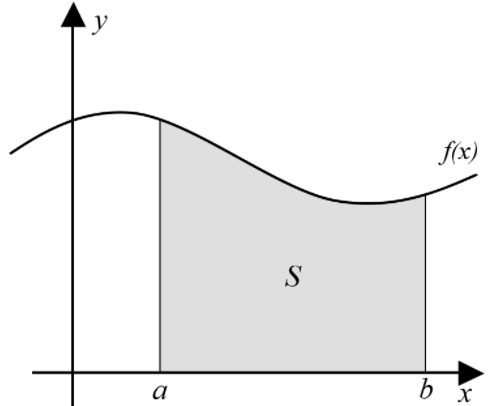
\includegraphics[width=0.8\textwidth]{./Imagens/Integral de Riemann/RI1.png} 
	\caption{Área sob a curva}
	\label{fig:RI1}
\end{figure}

\subsection{Integral de Riemann}

O valor total da área sob a curva da função $f(x)$ pode ser obtido dividindo essa área em diversos retângulos menores com extremidades nos pontos $[x_{0}, x_{1}, x_{2}, x_{3}, ..., x_{n}]$. A fórmula para a Integral de Rieman basicamente diz que a área da região compreendida entre o eixo horizontal e o gráfico da função $f(x)$, para x percorrendo o intervalo $[a,b]$, é igual ao limite da soma das áreas dos $n$ retângulos, quando o número desses retângulos tende a infinito.

\begin{figure}[H]
	\centering
	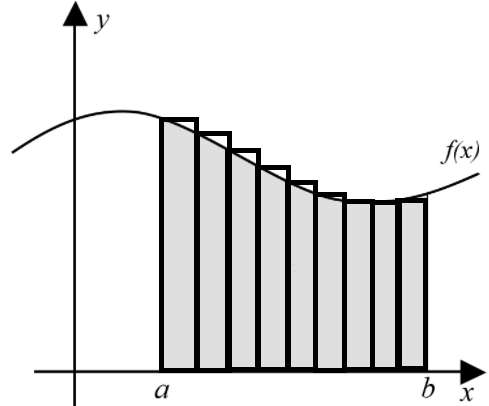
\includegraphics[width=0.8\textwidth]{./Imagens/Integral de Riemann/RI2.png} 
	\caption{Divisão da área}
	\label{fig:RI2}
\end{figure}

\subsubsection{Fórmula}

A Integral de Riemann da função $f(x)$ em relação a $x$ de $a$ para $b$ é: 

\[\large \int_{a}^{b}f(x) \; dx = \lim_{n \rightarrow \infty}\sum_{i=1}^{n} \frac{b-a}{n}f(x_{i-1})\]

A integral corresponde à "área com sinal", isto é, a área acima do eixo $x$ é positiva e a área abaixo do eixo $x$ é negativa.

Quando ela possui 2 limites, a integral é do tipo \textbf{definida}. Integral sem limite é denominada \textbf{indefinida}.

\subsection{Função primitiva/integral indefinida/antiderivada}

A \textbf{função primitiva/integral indefinida/antiderivada} de uma função $f$ é uma função diferenciável $F$ cuja derivada é igual à função original $f$. Isso pode ser representado simbolicamente por $F' = f$.

O processo de calcular funções primitivas (ou integrais indefinidas) de funções é oposto ao da diferenciação de funções, cujo objetivo é obter a derivada. Funções primitivas geralmente são representados por letras maiúsculas e estão relacionadas às integrais definidas pelo \textbf{Teorema Fundamental do Cálculo}.

Exemplo: 

A função $F(x) = \frac{x^3}{3}$ é a função primitiva de $f(x) = x^2$ uma vez que a derivada de $F(x) = \frac{x^3}{3}$ é $x^2$. Uma vez que a derivada de uma constante é zero, $x^2$ possuirá infinitas funções primitivas da forma $F(x) = \frac{x^3}{3} + C$ onde $C$ é denominada constante de integração.

\subsection{Teorema Fundamental do Cálculo}

O \textbf{Teorema Fundamental do Cálculo} diz que se $f(x)$ é uma função contínua em $[a,b]$, a sua integral definida nesse intervalo é a diferença entre as suas funções primitivas $F(x)$ nas extremidades desse intervalo:

\[\large \int_{b}^{a}f(x)\:dx = F(b) - F(a) = F(x)|^{b}_{a} \]

\subsection{Integral de Riemann utilizando scipy do Python}
Vamos utilizar a função **quad** da biblioteca Scipy para realizar a integração da função abaixo:

\[\large \int_{0}^{4}x^2dx\]

Para isso, vamos utilizar a função \textbf{lambda} do Python, que permite a criação de funções com número qualquer de argumentos:

\begin{minted}{python}
	x2 = lambda x: x**2
	print(x2)
	print(type(x2))
\end{minted}

Após isso, usamos a a função \textbf{integrate} da biblioteca \textbf{scipy} para realizar a integração.

O valor retornado pela função é uma tupla, onde o primeiro elemento é o valor estimado da integral e o segundo elemento é o limite superior de erro.

\begin{minted}{python}
	from scipy import integrate
	integrate.quad(x2, 0, 4)
\end{minted}

\[\large \int_{0}^{4}x^2dx \cong 21.333\]

\subsection{Exemplo por aproximação superior}

Vamos resolver a mesma integral de Riemann por aproximação superior. Para isso, vamos dividir a área S em diversos retângulos de base $[x_{i-1},x_{i}]$ e altura $f(x_{i})$

\begin{minted}{python}
import matplotlib.pyplot as plt
import numpy as np

fig, ax = plt.subplots(figsize =(8,6))

a = 0
b = 4
n = 5
x = np.linspace(a,b,n+1)

f = lambda x: x**2
vetor = []

for i in x:
	vetor.append(f(i))
	plt.vlines(i,0,f(i))

y = x**2
plt.plot(x,y)
plt.bar(x, vetor, align='edge', width=-(b-a)/n, 
color='pink')
plt.show()
\end{minted}

\begin{figure}[H]
	\centering
	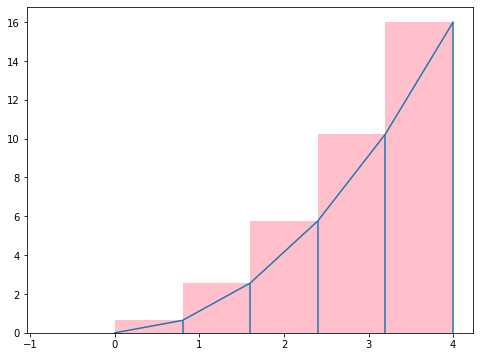
\includegraphics[width=0.8\textwidth]{./Imagens/Integral de Riemann/RI3.png} 
	\caption{Aproximação superior}
	\label{fig:RI3}
\end{figure}

A área da região S será tanto mais próxima do valor real $21.333$ quanto mais retângulos utilizarmos para dividir a área:

\begin{minted}{python}
import numpy as np

def area(a,b,n):
y = np.linspace(a,b,n+1)
w = (b - a)/n
f = lambda x: x**2
S = 0

for i in y[1:]:
	S = S + f(i)*w 
	
	print(f"Área: {S:.3f} (para {n} retângulos)")

area(0,4,5)
# Área: 28.160 (para 5 retângulos)
area(0,4,100)
# Área: 21.654 (para 100 retângulos)
area(0,4,500)
# Área: 21.397 (para 500 retângulos)
area(0,4,1000)
# Área: 21.365 (para 1000 retângulos)
area(0,4,5000)
# Área: 21.340 (para 5000 retângulos)
area(0,4,10000)
# Área: 21.337 (para 10000 retângulos)

\end{minted}

\subsection{Exemplo por aproximação inferior}

Vamos resolver a mesma integral de Riemann por aproximação inferior. Para isso, vamos dividir a área S em diversos retângulos de base $[x_{i-1},x_{i}]$ e altura $f(x_{i-1})$

\begin{minted}{python}
import matplotlib.pyplot as plt

fig, ax = plt.subplots(figsize =(8,6))

a = 0
b = 4
n = 5
x = np.linspace(a,b,n+1)

f = lambda x: x**2
vetor = []
for i in x:
	vetor.append(f(i))
	plt.vlines(i,0,f(i))

y = x**2
plt.plot(x,y)
plt.bar(x[:-1], vetor[:-1], align='edge', 
width=(b-a)/n, color='pink')
plt.show()
\end{minted}

\begin{figure}[H]
	\centering
	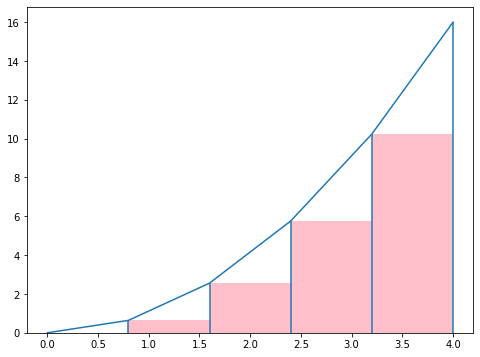
\includegraphics[width=0.8\textwidth]{./Imagens/Integral de Riemann/RI4.png} 
	\caption{Aproximação inferior}
	\label{fig:RI4}
\end{figure}

A área da região S será tanto mais próxima do valor real $21.333$ quanto mais retângulos utilizarmos para dividir a área:

\begin{minted}{python}
import numpy as np

def area(a,b,n):
y = np.linspace(a,b,n+1)
w = (b - a)/n
f = lambda x: x**2
S = 0

for i in y[:-1]:
	S = S + f(i)*w 

	print(f"Área: {S:.3f} (para {n} retângulos)")

area(0,4,5)
# Área: 15.360 (para 5 retângulos)
area(0,4,100)
# Área: 21.014 (para 100 retângulos)
area(0,4,500)
# Área: 21.269 (para 500 retângulos)
area(0,4,1000)
# Área: 21.301 (para 1000 retângulos)
area(0,4,5000)
# Área: 21.327 (para 5000 retângulos)
area(0,4,10000)
# Área: 21.330 (para 10000 retângulos)
\end{minted}

\subsection{Aplicações da Integral de Riemann}

\begin{itemize}
\item Pode ser utilizado na Matemática para: determinar a área de polígonos regulares ou irregulares; calcular a Transformada de Fourier; determinar o comprimento de uma curva; determinar o volume de um sólido.
\item Na física, é utilizado para: determinar a massa de um objeto caso a sua densidade seja conhecida; calcular o trabalho realizado partindo da força; calcular a velocidade e o instante dado a aceleração e as condições iniciais; calcular as equações de Maxwell.
\item Na engenharia é utilizado para determinar a força cortante e momento fletor; centroide de uma área; momento de inércia de uma área;
\item Na estatística é utilizado na função densidade de probabilidade.
\item Na química, pode ser utilizado para determinar a força a partir da pressão provocada por um conjunto de moléculas no interior de um recipiente.
\end{itemize}
